\documentclass[a4paper,11pt]{article}
\usepackage[utf8]{inputenc}
\usepackage[margin=1in]{geometry}
\usepackage[english, czech]{babel}
\usepackage{amsmath}

% package na vklad obrázků
\usepackage{graphicx}
\usepackage{caption}
\usepackage{subcaption}
\usepackage{stfloats} % opravuje obrázky přes celou stránku
\graphicspath{ {./images/} } % definování složky s obrázky

% zvyšování hloubky obsahu
\setcounter{tocdepth}{4}
\setcounter{secnumdepth}{4}

% citace
\usepackage[
    citestyle=numeric,
    autocite=superscript,
    sorting=none
    ]{biblatex} 
% \usepackage{biblatex}
\addbibresource{literature.bib}

% zajištujě závorky okolo citací
\DeclareCiteCommand{\supercite}[\mkbibsuperscript]
  {\iffieldundef{prenote}
     {}
     {\BibliographyWarning{Ignoring prenote argument}}%
   \iffieldundef{postnote}
     {}
     {\BibliographyWarning{Ignoring postnote argument}}%
   \bibopenbracket}%
  {\usebibmacro{citeindex}%
   \usebibmacro{cite}}
  {\supercitedelim}
  {\bibclosebracket}
  
% definování listings pro vklad kódu
\usepackage{listings}
\lstset{language=Java}

% abstrakt s větším písmem (https://tex.stackexchange.com/a/366170)
\makeatletter
\renewenvironment{abstract}{%
    \if@twocolumn
      \section*{\abstractname}%
    \else %% <- here I've removed \small
      \begin{center}%
        {\bfseries \Large\abstractname\vspace{\z@}}%  %% <- here I've added \Large
      \end{center}%
      \quotation
    \fi}
    {\if@twocolumn\else\endquotation\fi}
\makeatother

\selectlanguage{czech} % nastavení jazyka
\usepackage[T1]{fontenc}
% soubor k upřesnění rozdělení slov na slabiky

\hyphenation{Quick-sil-va}
\hyphenation{vše-chny}
\hyphenation{bom-by}
\hyphenation{ar-gu-men-tu-je}
\hyphenation{Au-to-swee-pe-ru} % upřesnění slabik v různých cizích slovech

\begin{document}


%%% -------------------- Titulní strana --------------------
\begin{titlepage}
\begin{center}
\large \vspace*{\fill}
\thispagestyle{empty}

\LARGE

{ \huge \textbf{Gymnázium Arabská, Praha 6, Arabská 14}}

{\LARGE Obor programování }

\vfill

\includegraphics{logogyarab.png}
\vspace{15pt}

\vfill

{\huge \textbf{Autosweeper}}

\vfill

Adam Suchý

\vfill

{\large Květen, 2021}

\vspace*{\fill}
\end{center}
\end{titlepage}

%%% -------------------- Prohlášení --------------------
\thispagestyle{empty}
\addtocounter{page}{-1}
\vspace*{\fill}
% TODO: Zeptat se profesora Lány, jestli nezle projekt publikovat pod MIT licencí
Prohlašuji, že jsem jediným autorem tohoto projektu, všechny citace jsou řádně označené a všechna 
použitá literatura a další zdroje jsou v práci uvedené. Tímto dle zákona 121/2000 Sb. (tzv. Autorský zákon) 
ve znění pozdějších předpisů uděluji bezúplatně škole Gymnázium, Praha 6, Arabská 14 oprávnění k výkonu 
práva na rozmnožování díla (§ 13) a práva na sdělování díla veřejnosti (§ 18) na dobu časově neomezenou a 
bez omezení územního rozsahu.
\bigskip

V .......... dne ............... \hspace{4cm} Adam Suchý ....................
\vspace{2cm}

%%% -------------------- Anotace --------------------
\newpage
\begin{abstract}
    Cílem tohoto ročníkového projektu je vytvořit hru, ve které je hráči ukázáno minové pole s úkolem ho
    zneškodnit. Hráč má za úkol najít všechny miny tím, že postupně odkrývá jednotlivá políčka. Při 
    každém odkrytí je hráči poskytnuta informace s množstvím min v okolních osmi políčkách. Když jsou 
    všechna políčka kromě min odhalena, tak hráč zvítězil. Jestliže hráč odhalí minu, je hra prohrána.
\end{abstract}

%%% -------------------- Obsah --------------------
\tableofcontents  % povinné strany

\twocolumn
\section{Úvod}
\subsection{Zadání projektu}
Autosweeper je variace na známou hru jménem Minesweeper, ve které se hledají miny. Hráč dostane libovolně velké dvourozměrné
pole \\čtverečků, pod kterými se můžou skrývat miny. Cílem hry je postupně odhalovat čtverečky pod kterými miny nejsou.
Při každém odhalení je hráči ukázáno číslo, které značí počet min v okolních osmi políčkách. Z těchto informací \\musí hráč hádat, jaké políčka může odhalit.

Součástí programu je automat, který hru umí řešit. Hráč si může vybrat mezi třemi \\herními módy: samostatný, s pomocí a
automatický. Když si hráč vybere samostatnou hru, tak se automat do hry nijak nezapojuje. Při hře s pomocí může hráč
kliknout na tlačítko "analyzovat", které automat spustí a ukáže hráči jaké políčka jsou vyhodnocena jako \\nebezpečná.
V automatickém módu automat řeší hru celou sám.

Při jakékoliv hře bude také běžet časovač, aby hráč mohl vidět své zlepšení, či zhoršení. Jestliže hru bude řešit
jen automat, tak bude časovač běžet jen při jeho "přemýšlení" neboli vyhodnocování nebezpečnosti políček.

\subsection{Hra Minesweeper a její historie}
Základní část programu Autosweeper je hra Minesweeper, prvně vydaná společností Microsoft v roce 1990 jako součást balíčku 
video her pro operační systém Windows 3.0. Avšak originální nápad této hry náleží video herní firmě Quicksilva a její hře
Mined-Out (1983) pro pročítače ZX Spectrum napsané v jazyce COBOL. Zatímco Mined-Out byla jediná doložená inspirace pro
Minesweeper, první hra s podobnou pointou byla Cube (1973) od Jerimaca Ratliffa. Princip hry Minesweeper byl tedy jeden z
nejstarších. Dokáže se vyrovnat například hře Tetris, nebo Pac-Man. \cite{minesweeperinfo}

\section{Tvorba hry}

\subsection{Uživatelské rozhraní}
Program je postaven na grafické knihovně\\ JavaFX pro programovací jazyk Java. Vzhledem k povaze hry je JavaFX zcela 
dostačující.

\subsubsection{Struktura}
% TODO: Přidat obrázky rozhraní
Celé uživatelské rozhraní se nachází ve dvou oknech. V prvním okně (obrázek \ref{fig:okno1}) uživatel najde hru 
společně s časovačem a dvěma až třemi tlačítky. Autosweeper lze používat jen s tímto jedním oknem, ale kdyby chtěl
uživatel změnit nastavení hry, může tak učinit ve druhém okně (obrázek \ref{fig:okno2}), které otevírá tlačítko
"settings". V nastavení lze změnit velikost pole, pravděpodobnost min a herní mód. Druhé okno je možné mít otevřené
pořád, nastavení se přenese vždy jen do příští hry, kterou začneme zmáčknutím smajlíku. Smajlík v prvním okně také
slouží jako indikátor stavu hry. (obrázek \ref{fig:stavy smajlíku})

    \begin{itemize}
        \item Okno 1
        \begin{itemize}
            \item Tlačítko se smajlíkem na restart hry, indikátor stavu hry
            \item Tlačítko na otevření nastavení
            \item Tlačítko na analýzu v módu s pomocí
            \item Herní pole
            \item Časovač
        \end{itemize}
        \item Okno 2
        \begin{itemize}
            \item Posuvník upravující šířku pole
            \item Posuvník upravující výšku pole
            \item Posuvník upravující pravděpodobnost výskytu min
            \item Tlačítko s výběrem herních módů
        \end{itemize}
    \end{itemize}

\begin{figure}
    \centering
    
\includegraphics[scale=0.6]{smiley.png}
    \caption{Všechny stavy smajlíku. Popisky (zleva doprava): Neutrální, Prohra, Hráč odhaluje minu, Výhra}
    \label{fig:stavy smajlíku}
\end{figure}

\begin{figure*}
    \centering
    \begin{subfigure}[b]{0.3\textwidth}
        \centering
        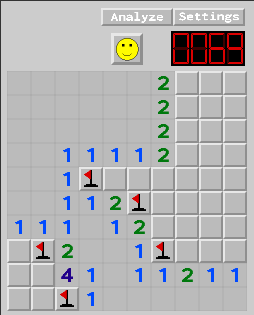
\includegraphics[scale=0.5]{images/okno1.png}
        \caption{Hlavní okno}
        \label{fig:okno1}
    \end{subfigure}
    \begin{subfigure}[b]{0.3\textwidth}
        \centering
        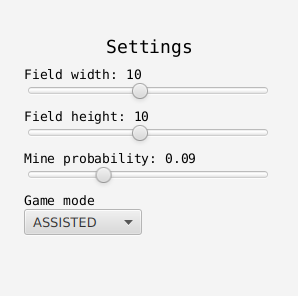
\includegraphics[scale=0.5]{images/okno2.png}
        \caption{Okno s nastavením}
        \label{fig:okno2}
    \end{subfigure}
    \caption{Okna s uživatelským rozhraním}
    \label{fig:okna}
\end{figure*}

\subsubsection{Design}
Vzhled programu je pokus o klon originálního designu Windows Minesweeper. Jako vzor byla použita jedna z mnoha
webových implementací \cite{playminesweeper}, jsou z ní vybrané zejména barvy čísel a vzhled smajlíku při
různých stavech hry. Původě mělo herní pole být tvořeno z několika tlačítek neboli objektů typu \\
{\tt javafx.scene.control.Button}, to by ale vyžadovalo hodně stylování a pravděpodobně také vytvořit si své
vlastní písmo s originálními číslicemi. Místo tlačítek jsou tedy využité \\{\tt javafx.scene.image.ImageView},
které umožňují zobrazit výstřižek obrázku. Na jednotlivé {\tt ImageView} jsou poté navázány funkce spouštějící
se při zmáčknutí, nebo puštění talčítka od myši.

Podobný problém nastal u časovače. Optimálně by měl být jeho sedmi-segmentovaný displej generován, ale moderní
počítače mají dost paměti na to, aby mohla každá číslice být uložená jako obrázek. Každá viditelná cifra je
stejně jako u všeho ostatního jeden {\tt ImageView}, všechny jsou poté spravovány třídou \\{\tt SevenSegmentDisplay}.

Všechny obrázky byly tvořeny mnou v programu Aseprite (Aseprite je placený, ale open-source. Je tedy zcela možné si
Aseprite zkompilovat zadarmo, což byla metoda, kterou jsem zvolil).

\subsection{Herní pole a stav hry}
Herní pole je hlavní částí programu. Poté co ho ovladač hlavního okna vytvoří, spravuje celou hru. Při inicializaci
nového pole ({\tt PlayingField}) je třeba poskytnout jen herní nastavení. Pole poté vygeneruje všechny políčka,
které lze dostat zpátky pomocí metody {\tt getCellAt}. Aby bylo možné pole rychle vykreslit,
je implementována metoda {\tt render}, která jako parametr dostane JavaFX {\tt GridPane}, do kterého
vloží \\všechny políčka.

\subsubsection{Komunikace mezi herním polem a hlavním ovladačem}
Po inicializaci pole a zavolání metody {\tt render} se vše odehrává uvnitř nově vytvořeného objektu.
Pro snadnou komunikaci s hlavním ovladačem a zajištění reagování ostatních prvků v uživatelském rozhraní existuje
systém událostí. Ovladač může použít metodu {\tt setEventHandler} pro nastavení funkce, která bude
naslouchat \\událostem ve hře. Například pří začátku hry nastane událost typu {\tt EventType.START}. 
Naslouchající funkce tuto událost zachytí a zapne časovač. Další herní události jsou například při odhalování políčka,
odhalení miny (= prohra), nebo při výhře.

\subsubsection{Stav hry}
V samotném objektu herního pole není uloženo moc informací. Jsou v něm uložené jen odkazy na jednotlivé políčka,
celkový počet bomb a počet neodhalených políček. Poslední dvě informace jsou potřeba jen při vyhodnocování,
jestli je hra dohraná, či ne. Většina informací o stavu hry jsou v jednotlivých políčkách, což jsou objekty třídy
{\tt Cell} (která dědí z již zmíněné třídy {\tt ImageView}). Každé políčko ukládá svou pozici, jestli je bomba, nebo
označené. Má také speciální hodnotu {\tt solver\_flags}, která slouží automatu k ukládání informací z minulých tahů,
a mnoho metod pro ulehčení práce s polem v automatu, nebo při vyhodnocování počtu bomb v okolí políčka. 

Jedna z výhod ukládání si informací rovnou v políčkách, které dědí z {\tt ImageView}, je možnost automatické aktualizace v uživatelském roz-\\hraní. Také se s takovými objekty jako s celky velmi dobře pracuje v automatu.
\begin{figure*}[hb!]
    \centering
    \begin{subfigure}[b]{0.3\textwidth}
        \centering
        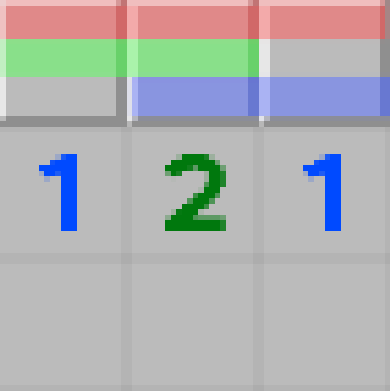
\includegraphics[scale=0.25]{images/uroven2-2.png}
        \caption{Situace z dvěmi bombami}
        \label{fig:situace_u2_dva}
    \end{subfigure}
    \begin{subfigure}[b]{0.3\textwidth}
        \centering
        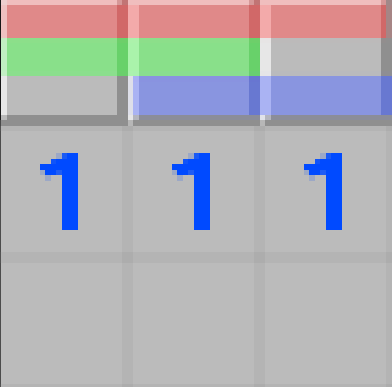
\includegraphics[scale=0.25]{images/uroven2-1.png}
        \caption{Situace s jednou bombou}
        \label{fig:situace_u2_jedna}
    \end{subfigure}
    \caption{Situace řešitelné 2. úrovní automatu}
    \label{fig:sitauce_u2}
\end{figure*}

\section{Automat}
Automat, který dokáže řešit hru, je hlavní odlišení projektu Autosweeper od původní hry. Algoritmus dostane jako vstupní data
herní pole a jeho stav přesně tak, jak je zobrazeno na obrazovce. Neví tedy, kde miny opravdu jsou a kde ne. Cíl automatu je
poté navrhnout možné tahy, které si myslí, že jsou bezpečné. Je strukturovaný do tří úrovní, každá se snaží najít možné tahy,
pokud žádný nenajde, je spuštěna další úroveň.

\subsection{První tah}
První tah hry se liší od ostatních tím, že je jisté, že není možné vydedukovat pozici žádné bomby. Nejdříve je nutné vyřešit
problém s rozlišením "začínající" hry od ostatních. Hra je pro automat začínající, jestliže se na herním poli nevyskytuje
žádná políčka s číslem (počtem \\bomb v okolí) 0 a počet odehraných tahů je méně než čtyři.

V této situaci automat odkrývá políčka v rozích, protože vzhledem k počtu okolních políček je nejvíce pravděpodobné, že stav
políčka nebude možné vydedukovat. \autocite{bercerra2015} Pravděpodo-\\bnost výhry se tím sice nezmění, ale algoritmus alespoň 
neplýtvá čas řešením hry, ve které bude muset hádat.

\subsection{První úroveň}
První úroveň automatu je algoritmus, který se dívá na stav každého odhaleného políčka a pokud se jeho číslo schoduje s počtem
neodhalených sousedů (8 sousedících políček), tak všechny sousedy označí jako bomby. Po zkontrolování celého pole jde zpátky na
začátek a prochází celé pole znovu. Hledá políčka, u kterých se jejich číslo schoduje s počtem nalezených bomb, jestliže taková
situace nastane, jsou odhaleni všichni sousedi, kteří nebyli označeni jako bomba.

Komplexitu prvního stupně odhaduji na \\$O(8n)$, jelikož pro každé políčko musí algoritmus zkontrolovat všech osm sousedů.
V praxi je ale vyhodnocování pole mnohem rychlejší vzhledem k počtu políček s číslem 0, které jsou pro výpočet zanedbatelné.

\begin{figure*}[ht!]
    \centering
    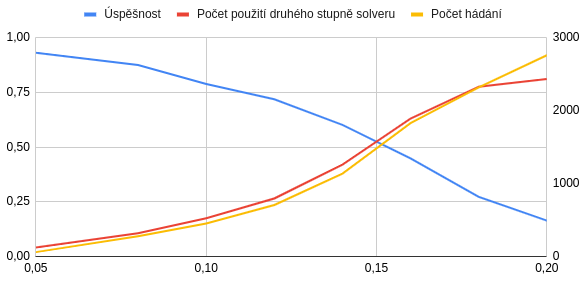
\includegraphics[scale=0.60]{images/uspesnost.png}
    \caption{Úspěšnost automatu na poli 20x20 pro různé obtížnosti hry}
    \label{fig:uspesnost}
\end{figure*}

\subsection{Druhá úroveň}
Druhá úroveň je spuštěna v případě, že první úroveň nic nenašla. Pracuje již s označenými bombami a snaží se vyřešit další
situace za pomocí spojení více neznámých políček do množin, neboli "kyblíků". Na obrázcích (\ref{fig:sitauce_u2}) lze vidět jakou
strukturu kyblíky mají. Červenou je označen kyblík prostřední číslice, levá číslice má zelený a pravá modrý. Červený kyblík je
hlavní, jelikož to je kyblík políčka, které se snažíme vyřešit. Všechny ostatní kyblíky musí být podmnožinou hlavního, abychom je
mohli od sebe odčítat. Tato limitace omezuje druhou úroveň na řešení situací 3x3. První úroveň tomuto velmi pomáhá, protože může
působení druhé úrovně rozšířit tím, že označí už odhalené bomby a zvýší tak šanci, že nějaký kyblík nebude přesahovat ven z
hlavního.

Poté co byly nalezeny všechny kyblíky a bylo zajištěno, že se mezi nimi nenachází žádné duplikáty, je potřeba vyřešit průniky
dvou, či více kyblíků. V situaci na obrázcích (\ref{fig:sitauce_u2}) se nachází jeden průnik a to mezi zeleným a modrým kyblíkem.
Algoritmus se nejdřív snaží najít jakékoliv políčko, které je ve více než jednom kyblíku. Pokud nějaké políčko najde, snaží se
dohledat celý průnik. Každý průnik poté zkusí vyhodnotit tím, že odečte očekávaný počet bomb v průniku od všech pronikajících
kyblíků včetně hlavního kyblíku. Jestliže součet vypočítaných hodnot je roven $0$, pak je v průniku bomba a jakékoliv jiné
políčko algoritmus považuje za bezpečné. Když součet naopak $0$ roven není, je třeba průnik ze všech pod-kyblíků odstranit bez
odčítání z celkového počtu bomb. Tedy průnik obsahuje všechny miny v hlavním kyblíku, jestliže následující rovnost platí:
\begin{equation*}
\sum_{x \in K} |x-\min K| = 0
\end{equation*}
Kde $K$ je množina počtů bomb všech pronikajících kyblíků a hlavního kyblíku.

Po ošetření průniků algoritmus odčítá všechny pod-kyblíky od hlavního (tzn. odstranit všechny políčka pod-kyblíku z hlavního
kyblíku a odečtení počtu bomb). Všechny zbylá políčka v hlavním kyblíku lze považovat za bezpečné za podmínky, že počet bomb se
rovná $0$. Při nerovnosti algoritmus výpočet zahodí a přechází na další políčko.


\subsection{Třetí úroveň}
Aby automat vždy navrhl nějaké políčko, je potřeba třetí úroveň. Tato úroveň se nesnaží vydedukovat bezpečné políčka, ale spočítá
jednoduchou pravděpodobnost bomby na každém políčku. Vzhledem k tomu, že výpočet pravé pravděpodobnosti výskytu bomby na políčku
je stejně těžký úkol jako samotné řešení, není pravděpodobnost z výpočtu pravdivá, ale jaksi orientační. Každé políčko dostane
pravděpodobnost jednoduchým výpočtem, který se provede pro každé odhalené políčko: $p = \frac{c}{n}$, kde $c$ je číslo na
odhaleném políčku a $n$ je počet neodhalených sousedů. V případě, že na jedno políčko bude víc pravděpodobností, algoritmus vybere
nejvyšší. Po výpočtu všech pravděpodobností algoritmus vybere políčko s nejmenší pravděpodobností výskytu bomby.


\subsection{Limity}
Autosweeper nedokáže vyřešit všechny Minesweeper hry. Řešení těchto her je těžký matematický problém. Richard Kaye ve své studii
nazvané "Minesweeper is NP-Complete" \\argumentuje mnoha způsoby, že Minesweeper problém je NP-úplný \autocite{Kaye2000}. To by
znamenalo, že je jeden z nejtěžších matematických problémů a jeho komplexita by byla stejná jako ta známého problému s obchodním
cestujícím \autocite{wiki_tsp}. \\Vždy úspěšný automat je hned vyloučen při prvním tahu, kdy je vždy možné narazit na minu. Záleží
tedy na implementaci hry, jestli první tah udělá zaručeně dobrým, nebo jestli herní pole bude už předgenerované (způsob používán
Autosweeperem).

Ve snaze kvantifikovat úspěšnost Autosweeperu byl spuštěn vždy na 1000 her pro různé nastavení a z výsledků se vytvořil graf
(obrázek \ref{fig:uspesnost}). Z grafu lze vidět, že automat má při jednoduché hře (pravděpodobnost výskytu min $0,05$) vysokou
úspěšnost a zároveň řeší většinu tahů jen pomocí prvního stupně. Při pravděpodobnosti $0,15$ je automat úspěšný jen v polovině
her. Tyto hry jsou těžké i pro lidské hráče. Při pravděpodobnosti $0,20$, tedy každé páté políčko je v průměru mina, automatu
selhává i druhý stupeň algoritmizace a můžeme vidět, že automat ve většině případech pouze neinformovaně hádá.



\section{Instalace}
Instalace Autosweeperu je poměrně jednoduchá. Postup k instalaci:
\begin{enumerate}
    \item Zkompilujte zdrojový kód, nebo si stáhněte zkompilovaný program z GitHubu
    \item Výsledný {\tt .jar} dejte společně s {\tt resources} do jedné složky
    \item Spusťte {\tt .jar} program
\end{enumerate}

\section{Závěr}
Myslím si, že se mi Autosweeper podařil. Uživatelské rozhraní je přesně takové, jaké jsem si představoval. Jediné z čeho jsem lehce
zklamaný je samotný automat. Původně jsem zamýšlel implementovat algoritmus popisovaný ve studii Bercerry \cite{bercerra2015}, ale
nechtěl jsem implementovat věc, které nerozumím. I přes lehké zklamání, že automat není 100\% úspěšný jsem rád, že umí vyřešit i
poměrně těžké hry. Na projektu by se dal zlepšit samotný automat, ale také i celková organizace kódu, jako například render políček,
který je sice velmi automatický, ale občas dělá neplechu.

\newpage
\onecolumn
\printbibliography
\listoffigures

\end{document}
